\newpage
\item Aumentar los precios de los productos de la subcategoría \textbf{Phones} en un 8\%.

\begin{lstlisting}
phones = σ subcategory = 'Phones' (products)

products = (products − phones)
         ∪ π productid, category, subcategory, price * 1.08 → price (phones)
\end{lstlisting}

Se actualizan los 184 productos de la subcategoría \texttt{Phones};
la relación \texttt{products} conserva sus 1862 renglones.
Las tuplas mostradas corresponden a los teléfonos ya actualizados
(\texttt{Phones}); se muestran por separado porque en la tabla general
de \texttt{products} los registros de \texttt{Phones} son muy escasos
(184 de 1862 renglones).

\begin{center}
  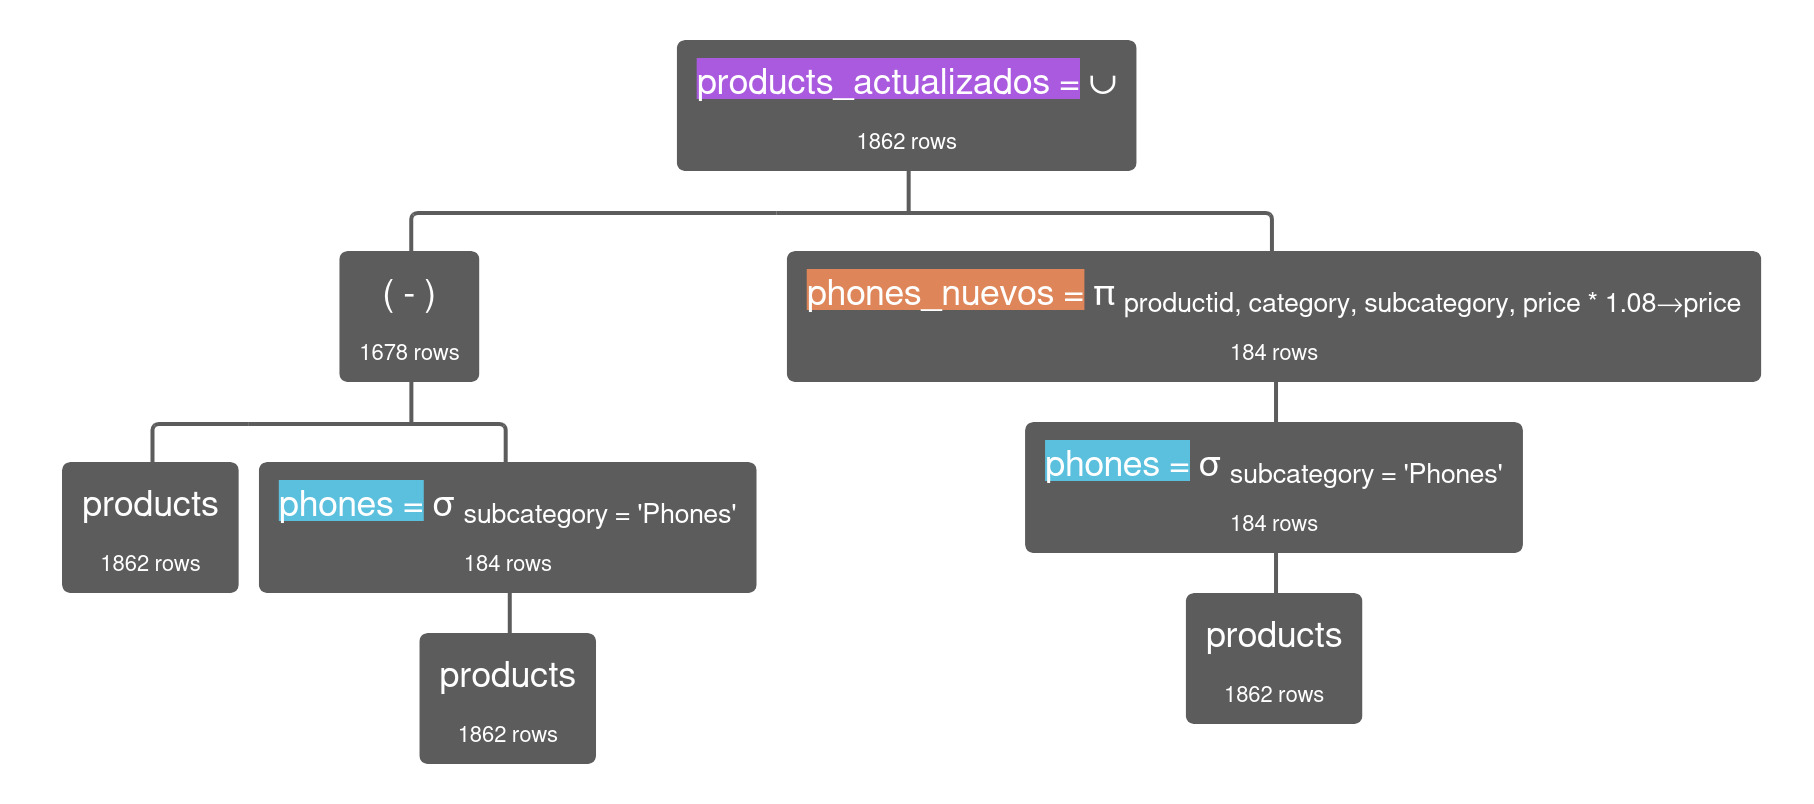
\includegraphics[width=0.72\textwidth]{figuras/3d_arbol.png}
\end{center}

\begin{center}
  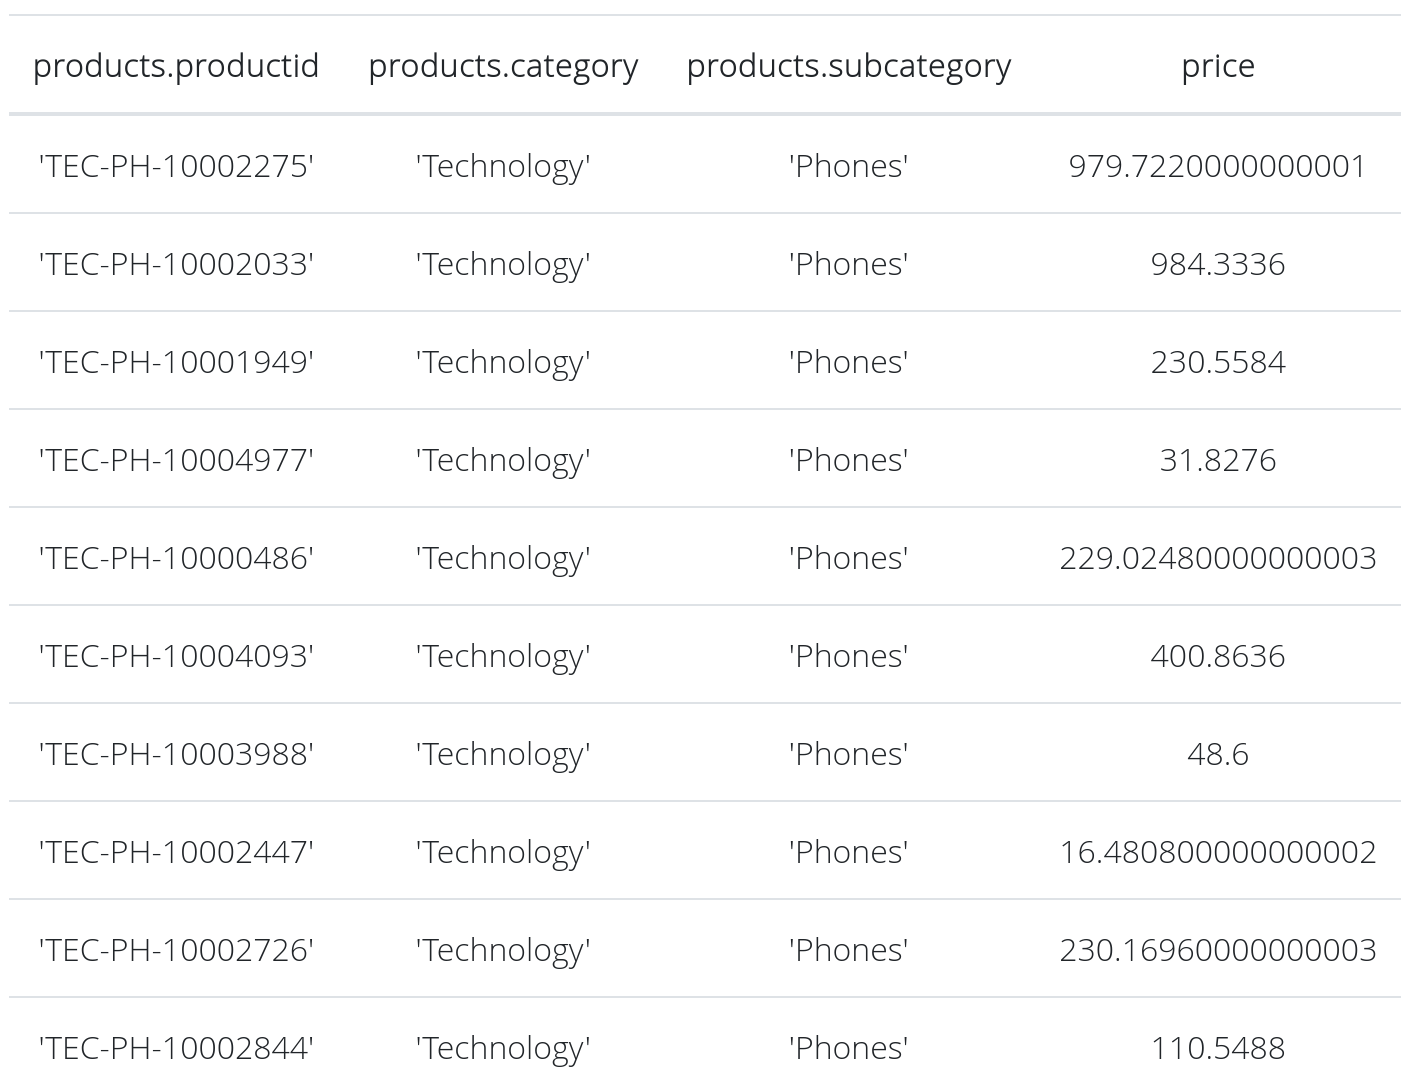
\includegraphics[width=0.55\textwidth]{figuras/3d_tuplas.png}
\end{center}
